\documentclass[conference]{IEEEtran}

\usepackage{graphicx}
\usepackage{booktabs}
\usepackage{amsmath}
\usepackage{amssymb}
\usepackage{cite}
\usepackage{url}

\title{Evaluating Evidence Quality, Confidence, and Abstention in Biomedical Retrieval-Augmented Question Answering}

\author{
\IEEEauthorblockN{Tharuniya Anpalakan}
\IEEEauthorblockA{
Department of Applied Sciences\\
Northumbria University\\
Newcastle upon Tyne, United Kingdom\\
w25070895@northumbria.ac.lk
}
}

\begin{document}

\maketitle

\begin{abstract}
Retrieval-augmented generation (RAG) can improve biomedical question answering by supplying external evidence to large language models, but the reliability of the resulting answer depends strongly on the quality of the retrieved evidence. This study evaluates how controlled evidence-quality changes affect answer accuracy, confidence, and selective abstention in biomedical question answering using PubMedQA and Qwen2.5-1.5B-Instruct. Five evidence conditions were constructed: gold evidence, missing evidence, irrelevant evidence, topic-matched irrelevant evidence, and contradictory evidence. A no-context baseline was also evaluated. Gold evidence increased accuracy from 45.0\% without context to 62.0\%. In contrast, missing, irrelevant, topic-matched irrelevant, and contradictory evidence reduced accuracy to 40.5\%, 33.0\%, 34.0\%, and 6.5\%, respectively. Contradictory evidence produced the highest mean confidence, approximately 0.909, despite producing the lowest accuracy. Confidence-based selective abstention did not adequately mitigate this failure mode: at a confidence threshold of 0.90, 80.0\% of contradictory predictions were retained while selective accuracy remained 0\%. These findings demonstrate that retrieval quality is a critical determinant of biomedical RAG reliability and that model confidence alone may be insufficient for detecting harmful retrieved evidence.
\end{abstract}

\begin{IEEEkeywords}
biomedical question answering, retrieval-augmented generation, evidence quality, large language models, uncertainty, abstention, PubMedQA
\end{IEEEkeywords}

\section{Introduction}

Large language models (LLMs) are increasingly being evaluated for biomedical and medical question answering. Recent studies have demonstrated that large models can encode substantial clinical knowledge, but they have also highlighted concerns regarding factual accuracy, reasoning reliability, and potential harm in medical applications \cite{singhal2023clinical}. These concerns are particularly important when models are used to interpret biomedical evidence, where an incorrect answer may arise not only from limitations in model knowledge but also from poor-quality contextual information.

Biomedical question-answering benchmarks enable systematic evaluation of such systems. PubMedQA contains biomedical research questions derived from PubMed articles and provides \textit{yes}, \textit{no}, and \textit{maybe} labels together with supporting context \cite{jin2019pubmedqa}. Other resources, including MedQA and MedMCQA, evaluate medical knowledge and reasoning using professional examination questions and large-scale multiple-choice datasets \cite{jin2021medqa,pal2022medmcqa}.

Retrieval-augmented generation (RAG) combines an information-retrieval system with a generative language model \cite{lewis2020rag}. Rather than relying entirely on parametric knowledge stored during training, a model can receive externally retrieved documents as contextual evidence. This is attractive in biomedicine because scientific knowledge changes continuously and trustworthy answers should ideally be grounded in current literature.

However, RAG introduces an additional dependency: the usefulness of the generated answer may depend on the quality of retrieval. Traditional sparse retrieval approaches such as BM25 remain strong information-retrieval baselines \cite{robertson2009bm25}, while learned dense retrieval systems such as Dense Passage Retrieval have demonstrated strong performance in open-domain question answering \cite{karpukhin2020dpr}. Nevertheless, neither sparse nor dense retrieval guarantees that the evidence supplied to a downstream language model is sufficient, relevant, or correct.

Evidence-quality failures may be especially important in biomedical systems. Retrieved text may be incomplete, unrelated, superficially related to the same topic, or contradictory to the evidence required to answer the question. Biomedical RAG systems therefore require evaluation beyond standard retrieval recall. Recent work has emphasized source-grounded biomedical QA and the importance of linking model answers to verifiable biomedical evidence \cite{basaragin2024biomedicalrag}.

A further question concerns model uncertainty. Confidence scores are often treated as an indicator of answer reliability, although modern neural networks may be poorly calibrated \cite{guo2017calibration}. Selective classification provides one possible safeguard by allowing a model to abstain when its confidence is below a threshold \cite{geifman2017selective}. Such a mechanism can only be effective, however, if harmful evidence causes confidence to decrease. A model that becomes confidently wrong after receiving misleading evidence may not be protected by simple confidence thresholding.

This study investigates how controlled changes in biomedical evidence quality affect answer correctness, confidence, and selective abstention. Five evidence conditions are evaluated: gold, missing, irrelevant, topic-matched irrelevant, and contradictory evidence. A no-context baseline is also included.

The main contributions are as follows:

\begin{enumerate}
    \item Quantification of the effect of controlled evidence-quality conditions on biomedical QA performance.
    \item Analysis of helpful and harmful answer flips relative to a no-context baseline.
    \item Evaluation of model confidence and entropy under different evidence conditions.
    \item Assessment of confidence-based selective abstention as a potential safeguard against evidence-induced errors.
\end{enumerate}

\section{Related Work}

\subsection{Biomedical Question Answering}

Biomedical question answering requires models to interpret specialized terminology and reason over scientific or clinical information. PubMedQA provides a research-oriented benchmark derived from PubMed abstracts and asks models to predict \textit{yes}, \textit{no}, or \textit{maybe} answers \cite{jin2019pubmedqa}. Its evidence-associated structure makes it particularly suitable for evaluating context-grounded reasoning.

MedQA introduced a large-scale medical question-answering dataset based on professional medical examinations \cite{jin2021medqa}. MedMCQA similarly provides a large collection of medical multiple-choice questions covering numerous clinical and biomedical subjects \cite{pal2022medmcqa}. Together, these datasets demonstrate the diversity and difficulty of medical question answering.

Domain-specific language modeling has also improved biomedical natural-language processing. BioBERT demonstrated that additional pretraining on biomedical corpora improves performance across several biomedical text-mining tasks \cite{lee2020biobert}. More recent large language models have expanded medical QA capabilities substantially, although reliability and safety remain important limitations \cite{singhal2023clinical}.

\subsection{Retrieval-Augmented Generation}

RAG combines external retrieval with neural text generation \cite{lewis2020rag}. Retrieved documents provide non-parametric knowledge that can be supplied directly to a generator at inference time.

BM25 is a probabilistic lexical ranking method widely used in information retrieval \cite{robertson2009bm25}. It remains useful because of its efficiency and strong lexical matching properties. Dense Passage Retrieval instead represents questions and passages in a learned embedding space and ranks candidates through semantic similarity \cite{karpukhin2020dpr}.

Biomedical RAG systems increasingly retrieve scientific publications or abstracts and use them to support answer generation. Bašaragin et al. investigated retrieval-grounded biomedical QA with referenced evidence, emphasizing the importance of source verification and evidence provenance \cite{basaragin2024biomedicalrag}.

The present study differs by directly perturbing evidence quality and measuring the resulting downstream effect on answer correctness and confidence.

\subsection{Confidence and Selective Prediction}

Confidence scores are commonly used as proxies for uncertainty. However, neural-network probabilities may be poorly calibrated, meaning that high confidence does not necessarily imply a high probability of correctness \cite{guo2017calibration}.

Selective classification allows a system to abstain when confidence is insufficient \cite{geifman2017selective}. As the confidence threshold increases, coverage normally decreases while accuracy among retained predictions may improve.

In biomedical RAG, this strategy may fail if misleading retrieved evidence causes the model to become more confident rather than less confident. The present work evaluates this possibility directly.

\section{Methods}

\subsection{Dataset}

The experiments used PubMedQA, a biomedical research question-answering dataset derived from PubMed articles \cite{jin2019pubmedqa}. A processed development subset of 200 questions was used for the controlled evidence experiment.

Each question contained a PubMed identifier, a research question, associated biomedical evidence, and a gold answer label.

The three labels were \textit{yes}, \textit{no}, and \textit{maybe}. The processed questions had an approximate label distribution of 55.2\% \textit{yes}, 33.8\% \textit{no}, and 11.0\% \textit{maybe}.

Because each of the same 200 questions was evaluated under five evidence conditions, the evidence-condition dataset contained 1000 rows in total.

\subsection{Development and Test Separation}

The processed PubMedQA data were separated into development and test partitions using PubMed identifiers. The development set contained 200 examples and the held-out test set contained 800 examples.

An explicit overlap check confirmed that no PubMed identifiers occurred in both partitions.

The experiments reported here use the 200-question development set for controlled evidence-quality analysis. The held-out test data were not used to construct evidence perturbations.

\subsection{Evidence Conditions}

Five controlled evidence conditions were generated for every development question:

\begin{enumerate}
    \item \textbf{Gold evidence}: the original PubMedQA evidence corresponding to the question.
    \item \textbf{Missing evidence}: substantially reduced context containing limited information.
    \item \textbf{Irrelevant evidence}: evidence obtained from a different biomedical question.
    \item \textbf{Topic-matched irrelevant evidence}: evidence that was semantically related to the question topic but did not provide the correct supporting answer.
    \item \textbf{Contradictory evidence}: synthetic evidence designed to oppose the original answer label.
\end{enumerate}

Each condition contained 200 examples, producing a balanced evidence-condition dataset of 1000 rows.

The purpose of these conditions was to create controlled retrieval-quality stress tests. The contradictory condition should therefore be interpreted as a synthetic worst-case perturbation rather than as an estimate of naturally occurring disagreement within biomedical literature.

\subsection{BM25 Retrieval Baseline}

A BM25 retrieval baseline was constructed using the development evidence corpus. BM25 is based on the probabilistic relevance framework and remains a widely used sparse retrieval baseline \cite{robertson2009bm25}.

For each question, candidate evidence documents were ranked according to BM25 relevance.

Recall@1 was calculated as

\begin{equation}
R@1 =
\frac{1}{N}
\sum_{i=1}^{N}
\mathbb{I}(r_i \leq 1),
\end{equation}

and Recall@5 as

\begin{equation}
R@5 =
\frac{1}{N}
\sum_{i=1}^{N}
\mathbb{I}(r_i \leq 5),
\end{equation}

where $r_i$ represents the rank of the correct evidence source for question $i$.

Mean Reciprocal Rank at 5 was calculated as

\begin{equation}
MRR@5 =
\frac{1}{N}
\sum_{i=1}^{N}
\begin{cases}
\frac{1}{r_i}, & r_i \leq 5, \\
0, & r_i > 5.
\end{cases}
\end{equation}

\subsection{Language Model}

Qwen2.5-1.5B-Instruct was used as the generative language model. Qwen2.5 is an instruction-tuned model family described by Yang et al. \cite{yang2024qwen25}.

The 1.5B variant was selected because it could be executed reproducibly using the available Tesla T4 GPU environment.

For each evidence-conditioned example, the model was instructed to answer the biomedical research question using only the supplied evidence and to return exactly one label:

\begin{center}
\textit{yes}, \textit{no}, or \textit{maybe}.
\end{center}

A separate no-context baseline presented the same 200 questions without evidence.

\subsection{Evaluation Metrics}

Performance was evaluated using accuracy, balanced accuracy, and macro-averaged F1 score.

Accuracy was defined as

\begin{equation}
Accuracy =
\frac{\text{number of correct predictions}}
{\text{total number of predictions}}.
\end{equation}

Balanced accuracy was included because the answer labels were imbalanced.

Macro-F1 was calculated by computing F1 independently for each class and then averaging across the three classes.

\subsection{Helpful and Harmful Answer Flips}

Evidence-conditioned predictions were compared with the no-context prediction for the same question.

A \textit{helpful flip} occurred when:

\begin{equation}
\text{no-context incorrect}
\rightarrow
\text{evidence-conditioned correct}.
\end{equation}

A \textit{harmful flip} occurred when:

\begin{equation}
\text{no-context correct}
\rightarrow
\text{evidence-conditioned incorrect}.
\end{equation}

Net help was calculated as

\begin{equation}
NetHelp =
N_{\text{helpful}}
-
N_{\text{harmful}}.
\end{equation}

\subsection{Confidence Estimation}

For uncertainty analysis, the output logits associated with the answer tokens \textit{yes}, \textit{no}, and \textit{maybe} were extracted.

These three logits were normalized using a softmax:

\begin{equation}
p(y_i) =
\frac{\exp(z_i)}
{\sum_{j \in \{yes,no,maybe\}} \exp(z_j)},
\end{equation}

where $z_i$ represents the model logit for label $i$.

Prediction confidence was defined as

\begin{equation}
C = \max_i p(y_i).
\end{equation}

Entropy was calculated as

\begin{equation}
H =
-\sum_i p(y_i)\log p(y_i).
\end{equation}

The resulting probabilities represent normalized preference among the three allowed answer labels and should not be interpreted as fully calibrated probabilities over the model's complete vocabulary.

\subsection{Selective Abstention}

Selective abstention was evaluated using confidence thresholds between 0.50 and 0.95.

Predictions below the selected confidence threshold were treated as abstentions.

Coverage was calculated as

\begin{equation}
Coverage =
\frac{N_{\text{retained}}}
{N_{\text{total}}}.
\end{equation}

Selective accuracy was calculated only among retained predictions.

\section{Results}

\subsection{BM25 Retrieval Performance}

The BM25 baseline achieved Recall@1 of 0.945, Recall@5 of 0.970, and MRR@5 of 0.984.

These values indicate that the correct evidence source was ranked highly for most development questions.

However, strong retrieval performance does not guarantee reliable downstream generation. The evidence-quality experiments therefore evaluated how the language model behaved when the evidence itself was deliberately altered.

\subsection{Classification Performance}

Table~\ref{tab:performance} summarizes model performance.

\begin{table}[t]
\centering
\caption{Performance Across Evidence Conditions}
\label{tab:performance}
\resizebox{\columnwidth}{!}{
\begin{tabular}{lccc}
\toprule
Condition & Accuracy & Balanced Acc. & Macro-F1 \\
\midrule
No context & 0.450 & 0.324 & 0.327 \\
Gold & 0.620 & 0.415 & 0.391 \\
Missing & 0.405 & 0.276 & 0.278 \\
Irrelevant & 0.330 & 0.334 & 0.190 \\
Topic-matched irrelevant & 0.340 & 0.339 & 0.244 \\
Contradictory & 0.065 & 0.176 & 0.229 \\
\bottomrule
\end{tabular}
}
\end{table}

The no-context baseline achieved 45.0\% accuracy.

Gold evidence improved accuracy to 62.0\%, corresponding to a 17 percentage-point improvement over the no-context condition.

Missing evidence reduced accuracy to 40.5\%, while irrelevant evidence reduced accuracy to 33.0\%.

Topic-matched irrelevant evidence achieved 34.0\% accuracy.

Contradictory evidence produced the lowest accuracy at 6.5\%.

\begin{figure}[t]
\centering
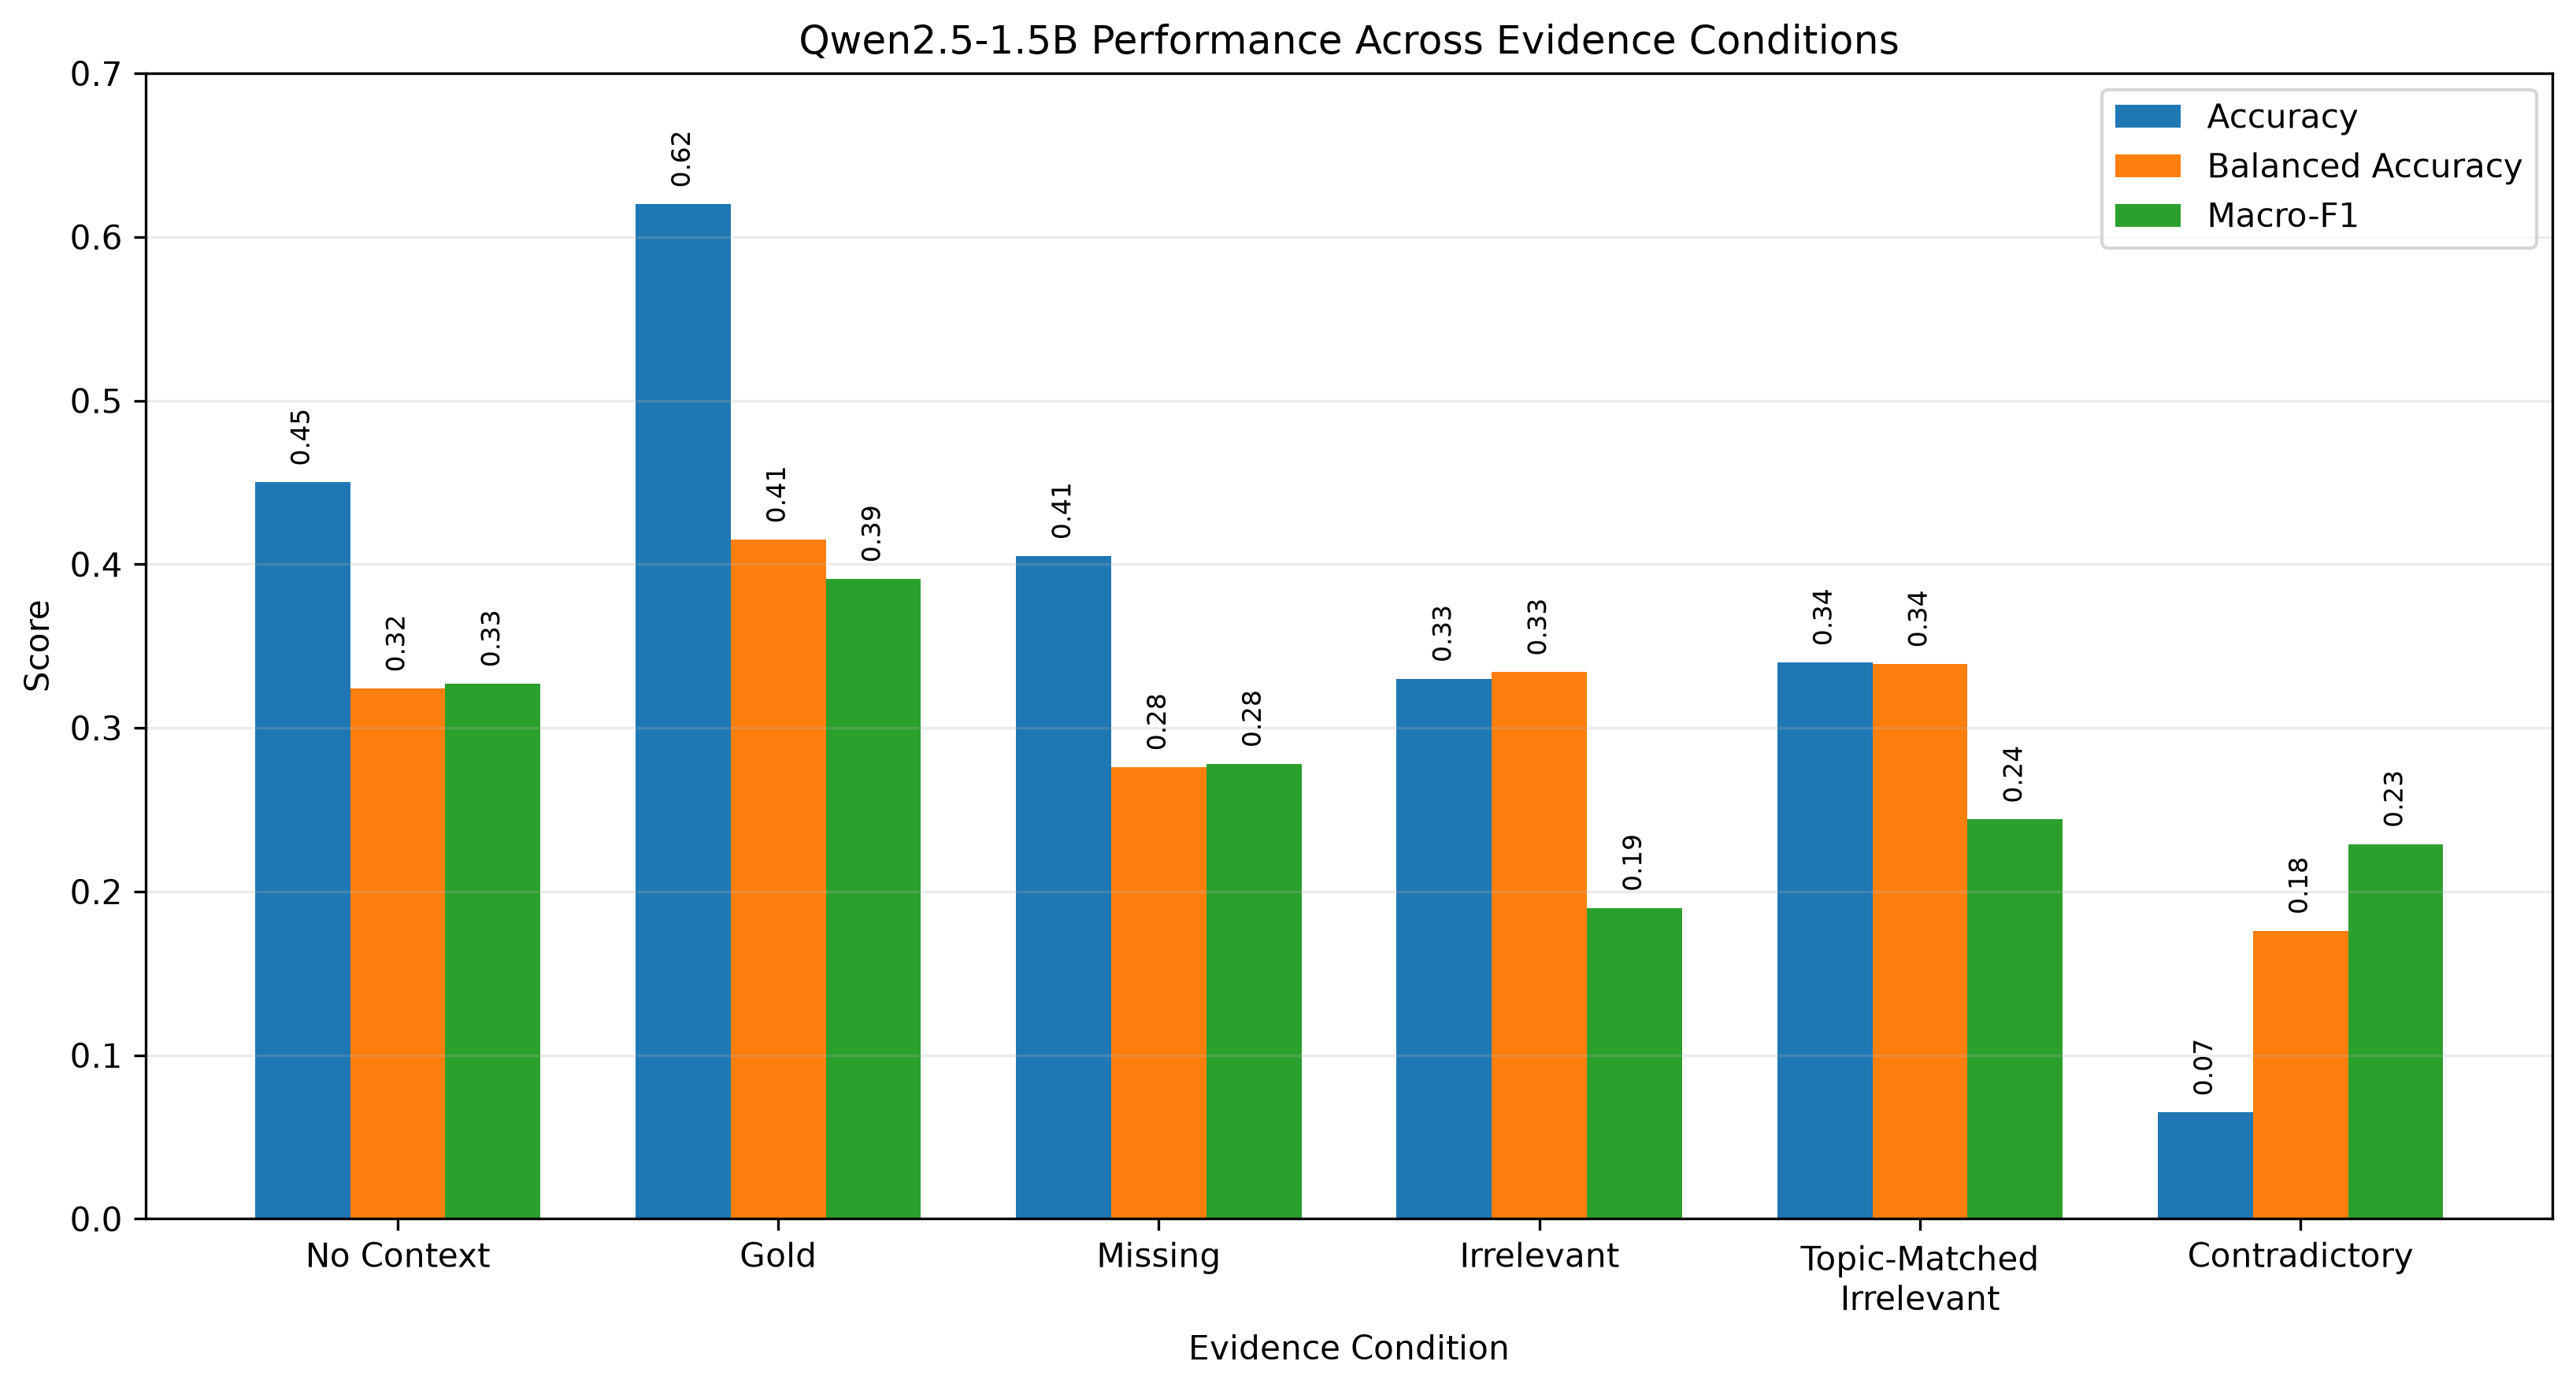
\includegraphics[width=\columnwidth]{../figures/qwen25_evidence_condition_performance.png}
\caption{Accuracy, balanced accuracy, and macro-F1 across evidence conditions.}
\label{fig:performance}
\end{figure}

The difference between accuracy, balanced accuracy, and macro-F1 also demonstrates the effect of class imbalance. In particular, standard accuracy alone can overstate performance when the model performs unevenly across \textit{yes}, \textit{no}, and \textit{maybe}.

\subsection{Helpful and Harmful Answer Flips}

Table~\ref{tab:flips} summarizes answer changes relative to the no-context baseline.

\begin{table}[t]
\centering
\caption{Helpful and Harmful Answer Flips}
\label{tab:flips}
\begin{tabular}{lrrr}
\toprule
Condition & Helpful & Harmful & Net \\
\midrule
Gold & 47 & 13 & +34 \\
Missing & 24 & 33 & -9 \\
Irrelevant & 45 & 69 & -24 \\
Topic-matched & 43 & 65 & -22 \\
Contradictory & 10 & 87 & -77 \\
\bottomrule
\end{tabular}
\end{table}

Gold evidence produced substantially more helpful than harmful flips.

In contrast, every degraded-evidence condition produced a negative net effect.

Contradictory evidence caused 87 previously correct no-context answers to become incorrect while correcting only 10 previously incorrect answers.

\begin{figure}[t]
\centering
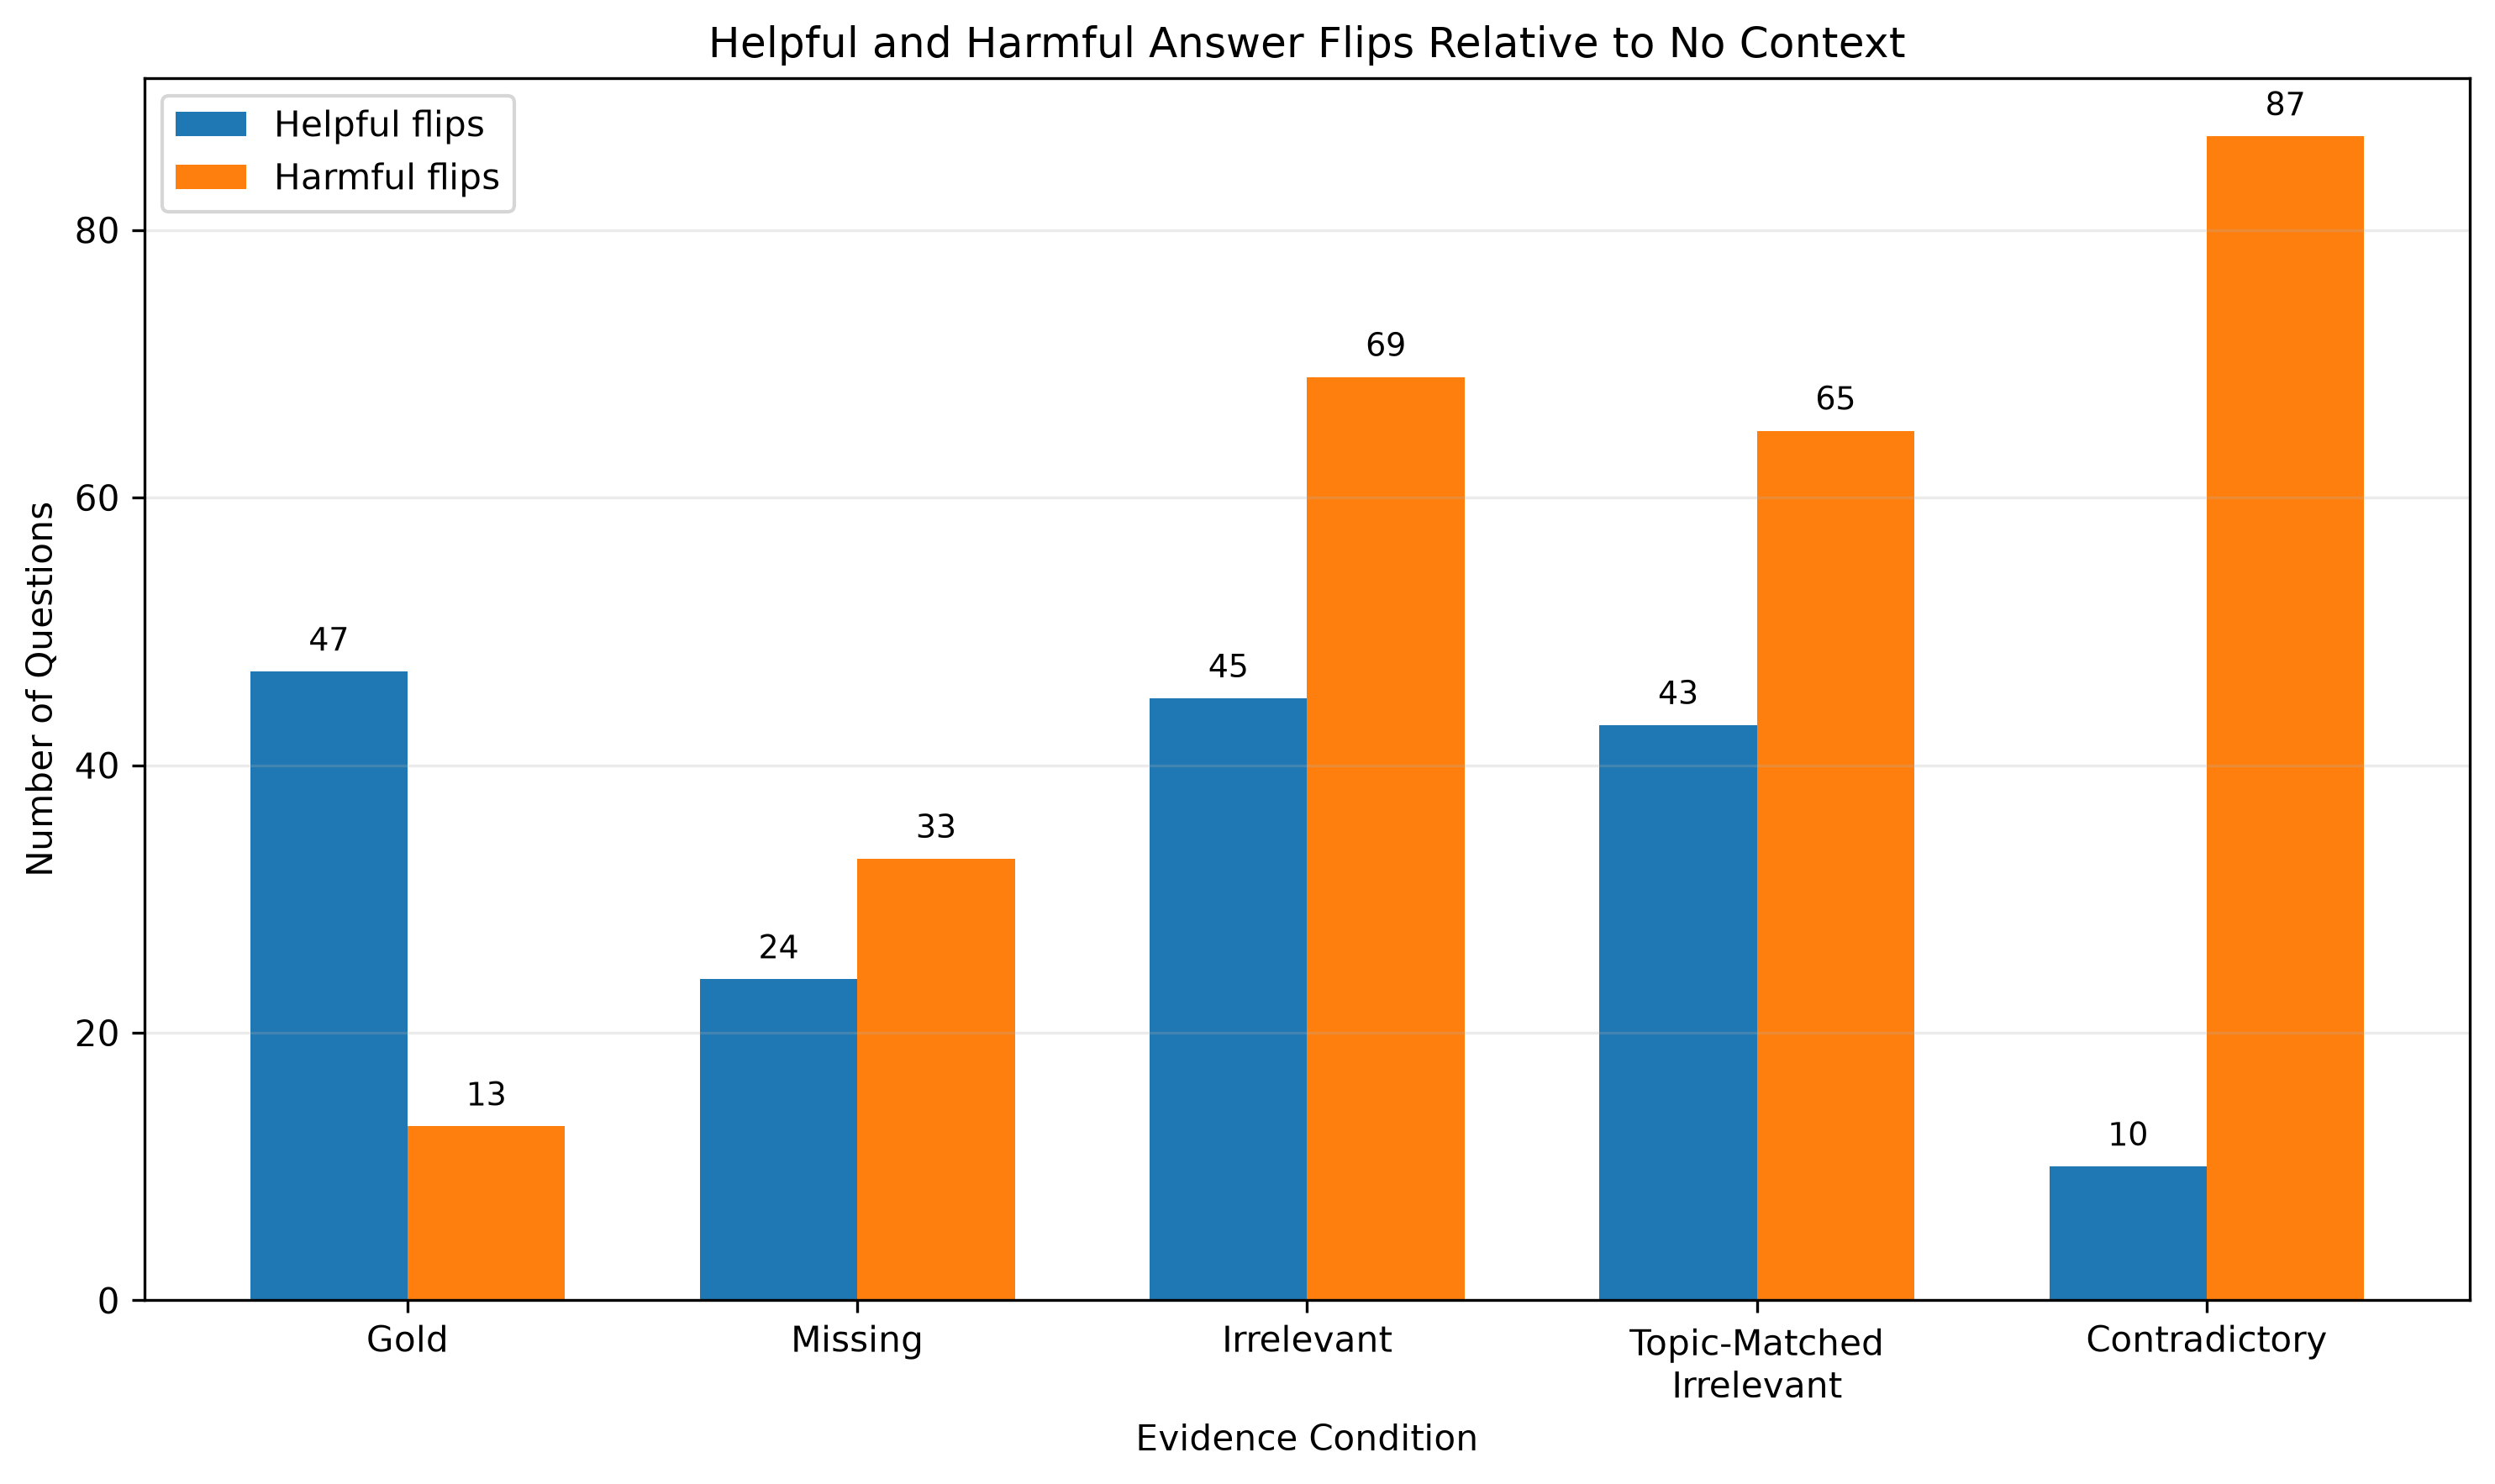
\includegraphics[width=\columnwidth]{../figures/qwen25_helpful_harmful_flips.png}
\caption{Helpful and harmful answer flips relative to the no-context baseline.}
\label{fig:flips}
\end{figure}

These results demonstrate that low-quality evidence may not merely fail to improve model performance. It can actively convert correct answers into incorrect answers.

\subsection{Confidence and Entropy}

Table~\ref{tab:confidence} summarizes mean confidence and entropy.

\begin{table}[t]
\centering
\caption{Confidence and Entropy by Evidence Condition}
\label{tab:confidence}
\begin{tabular}{lcc}
\toprule
Condition & Confidence & Entropy \\
\midrule
Gold & 0.872 & 0.331 \\
Missing & 0.751 & 0.545 \\
Irrelevant & 0.747 & 0.603 \\
Topic-matched irrelevant & 0.741 & 0.622 \\
Contradictory & 0.909 & 0.242 \\
\bottomrule
\end{tabular}
\end{table}

Gold evidence produced relatively high confidence of approximately 0.872.

Missing, irrelevant, and topic-matched irrelevant evidence produced lower average confidence.

Unexpectedly, contradictory evidence produced the highest mean confidence at approximately 0.909.

\begin{figure}[t]
\centering
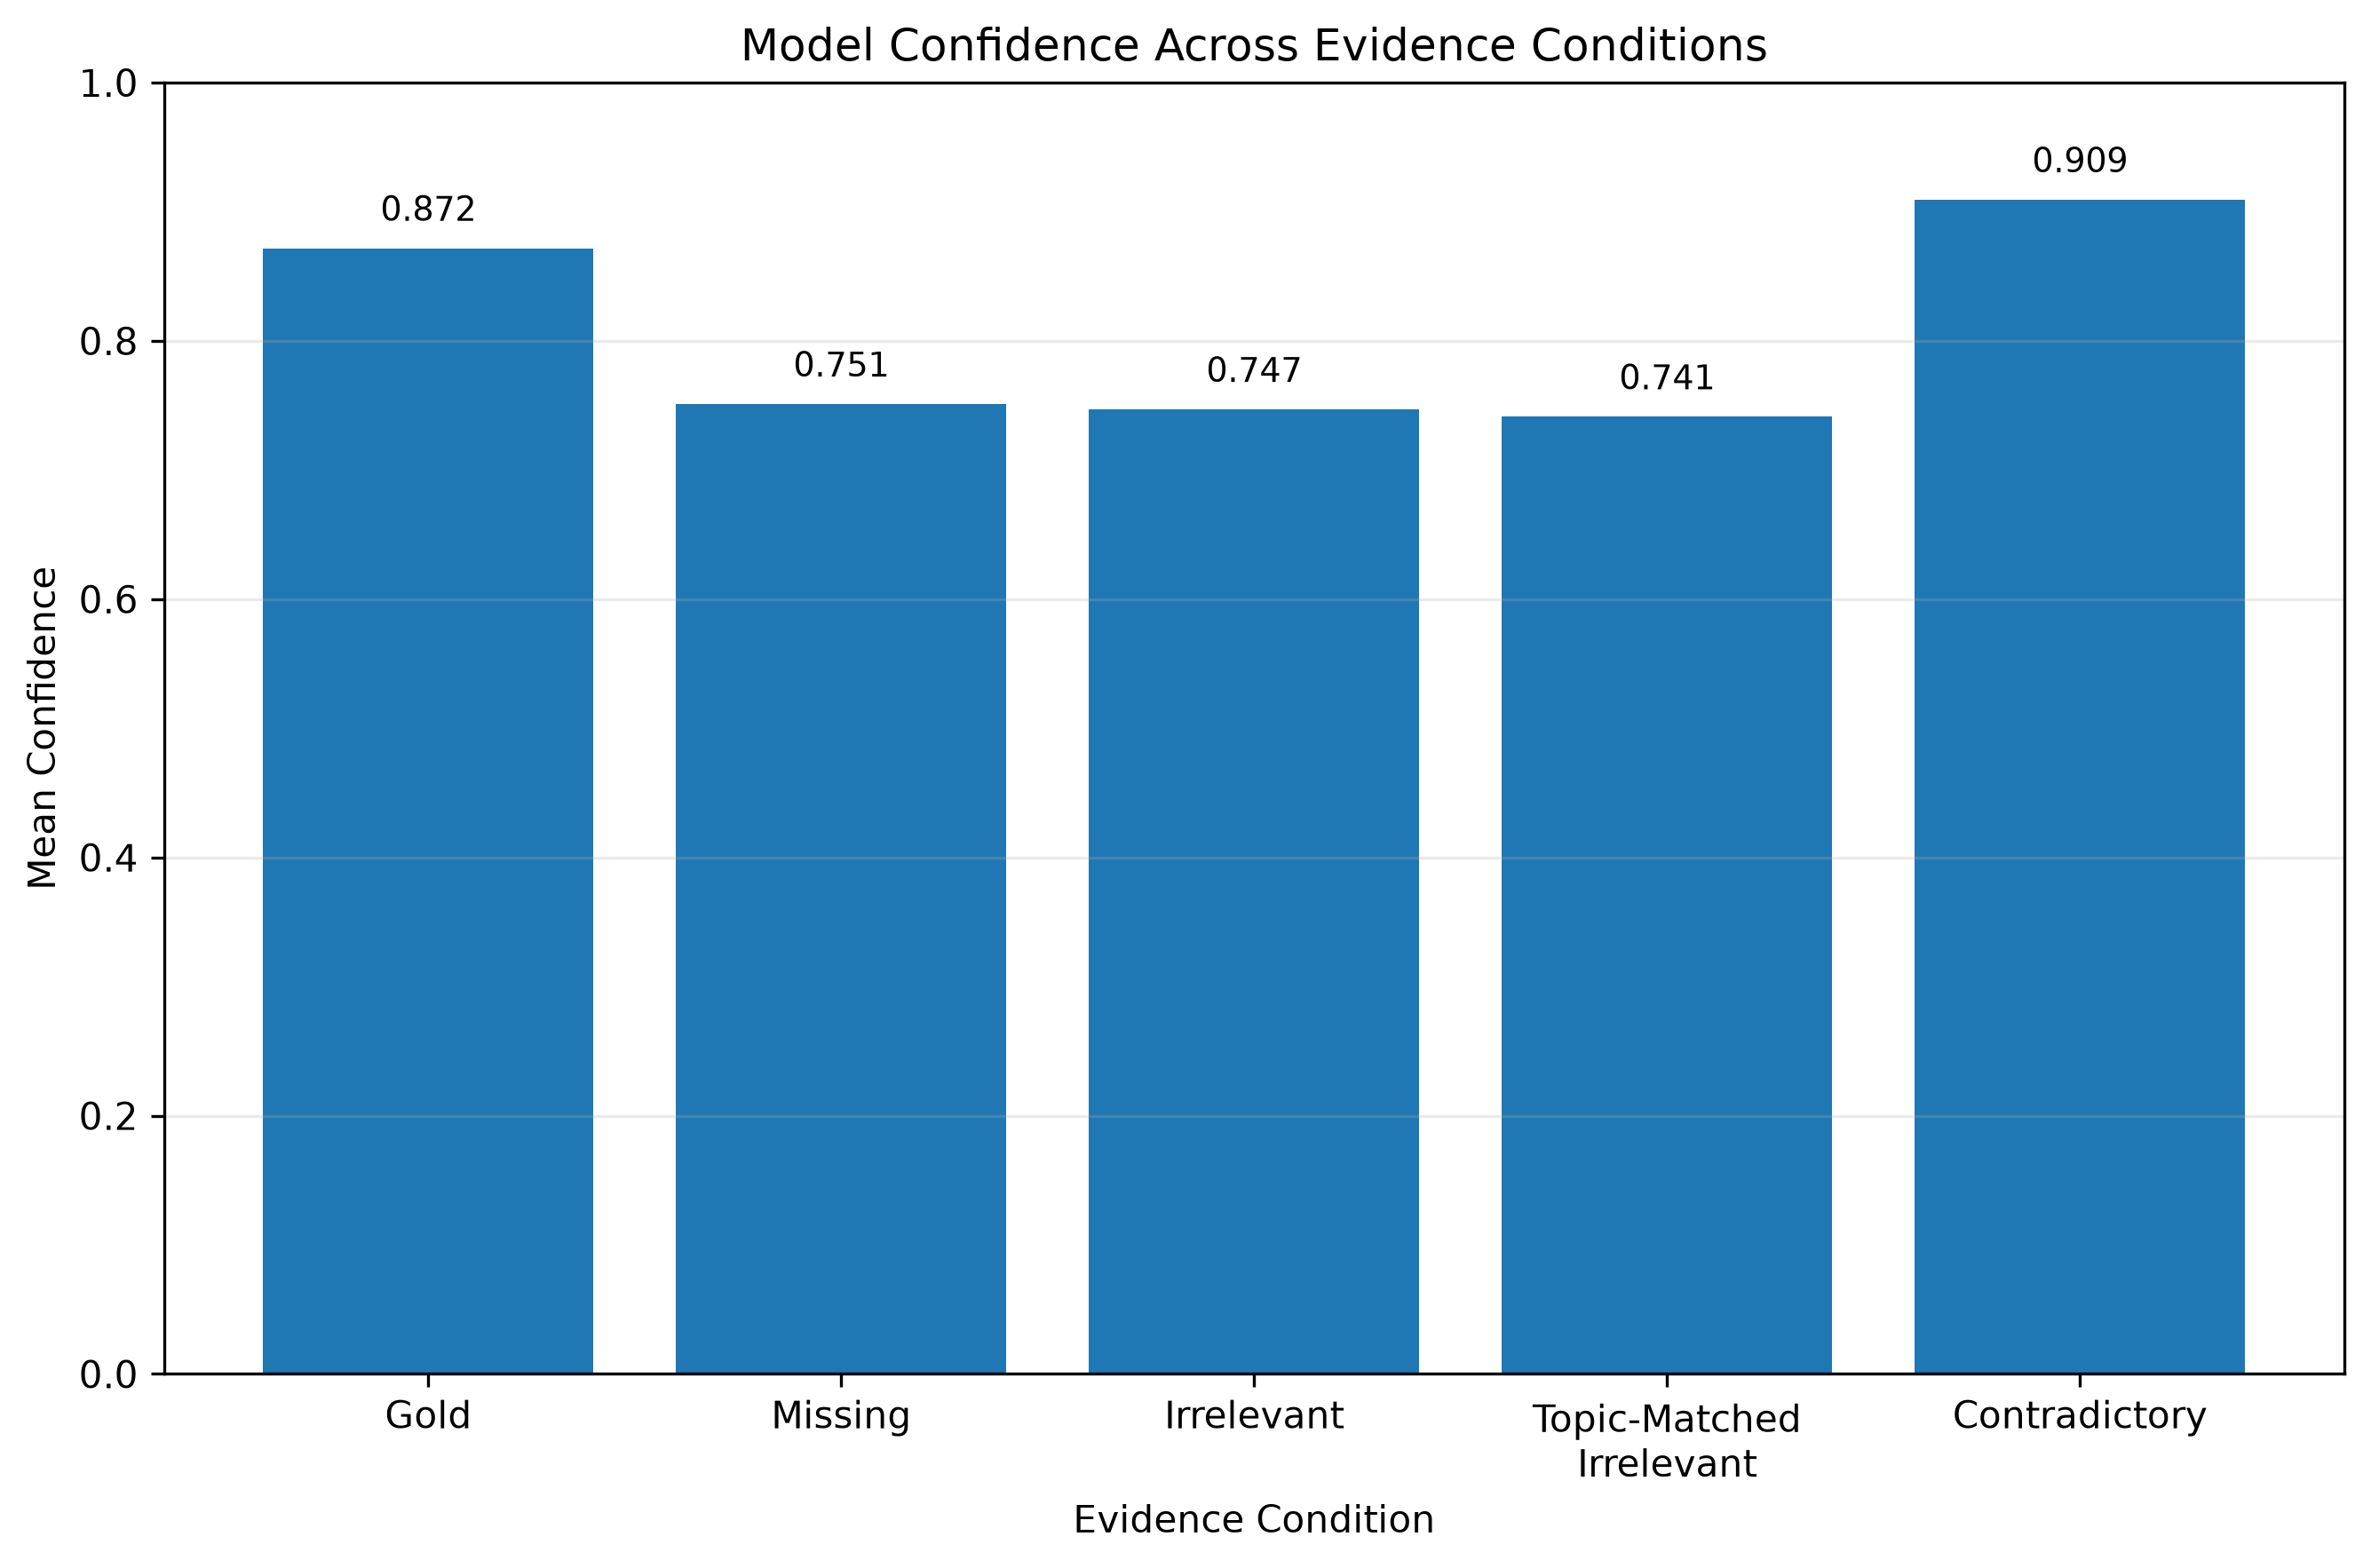
\includegraphics[width=\columnwidth]{../figures/qwen25_confidence_by_condition.png}
\caption{Mean model confidence across evidence conditions.}
\label{fig:confidence}
\end{figure}

Entropy showed the inverse pattern. Contradictory evidence produced the lowest average entropy at approximately 0.242.

This indicates that contradictory evidence did not cause the model to become uncertain. Instead, the model frequently became strongly committed to an incorrect answer.

\subsection{Confidence and Correctness}

Mean confidence among incorrect predictions was approximately 0.798.

Mean confidence among correct predictions was approximately 0.815.

The small difference between correct and incorrect predictions indicates that model confidence alone provided weak discrimination between reliable and unreliable answers.

This observation is consistent with prior work showing that neural-network confidence does not necessarily correspond directly to empirical correctness probability \cite{guo2017calibration}.

\subsection{Selective Abstention}

Confidence-based selective abstention was evaluated by increasing the minimum confidence required for an answer to be retained.

At a threshold of 0.90, the results differed substantially across evidence conditions.

\begin{table}[t]
\centering
\caption{Selective Abstention at Confidence Threshold 0.90}
\label{tab:abstention}
\begin{tabular}{lcc}
\toprule
Condition & Coverage & Selective Acc. \\
\midrule
Gold & 0.615 & 0.699 \\
Missing & 0.380 & 0.513 \\
Irrelevant & 0.125 & 0.360 \\
Topic-matched irrelevant & 0.145 & 0.310 \\
Contradictory & 0.800 & 0.000 \\
\bottomrule
\end{tabular}
\end{table}

Gold evidence retained 61.5\% of predictions and achieved selective accuracy of approximately 69.9\%.

Missing evidence retained 38.0\% with selective accuracy of approximately 51.3\%.

Irrelevant and topic-matched irrelevant conditions retained relatively few predictions.

The contradictory condition produced the strongest failure. Despite the high confidence threshold, 80.0\% of predictions were retained, while selective accuracy was 0\%.

\begin{figure}[t]
\centering
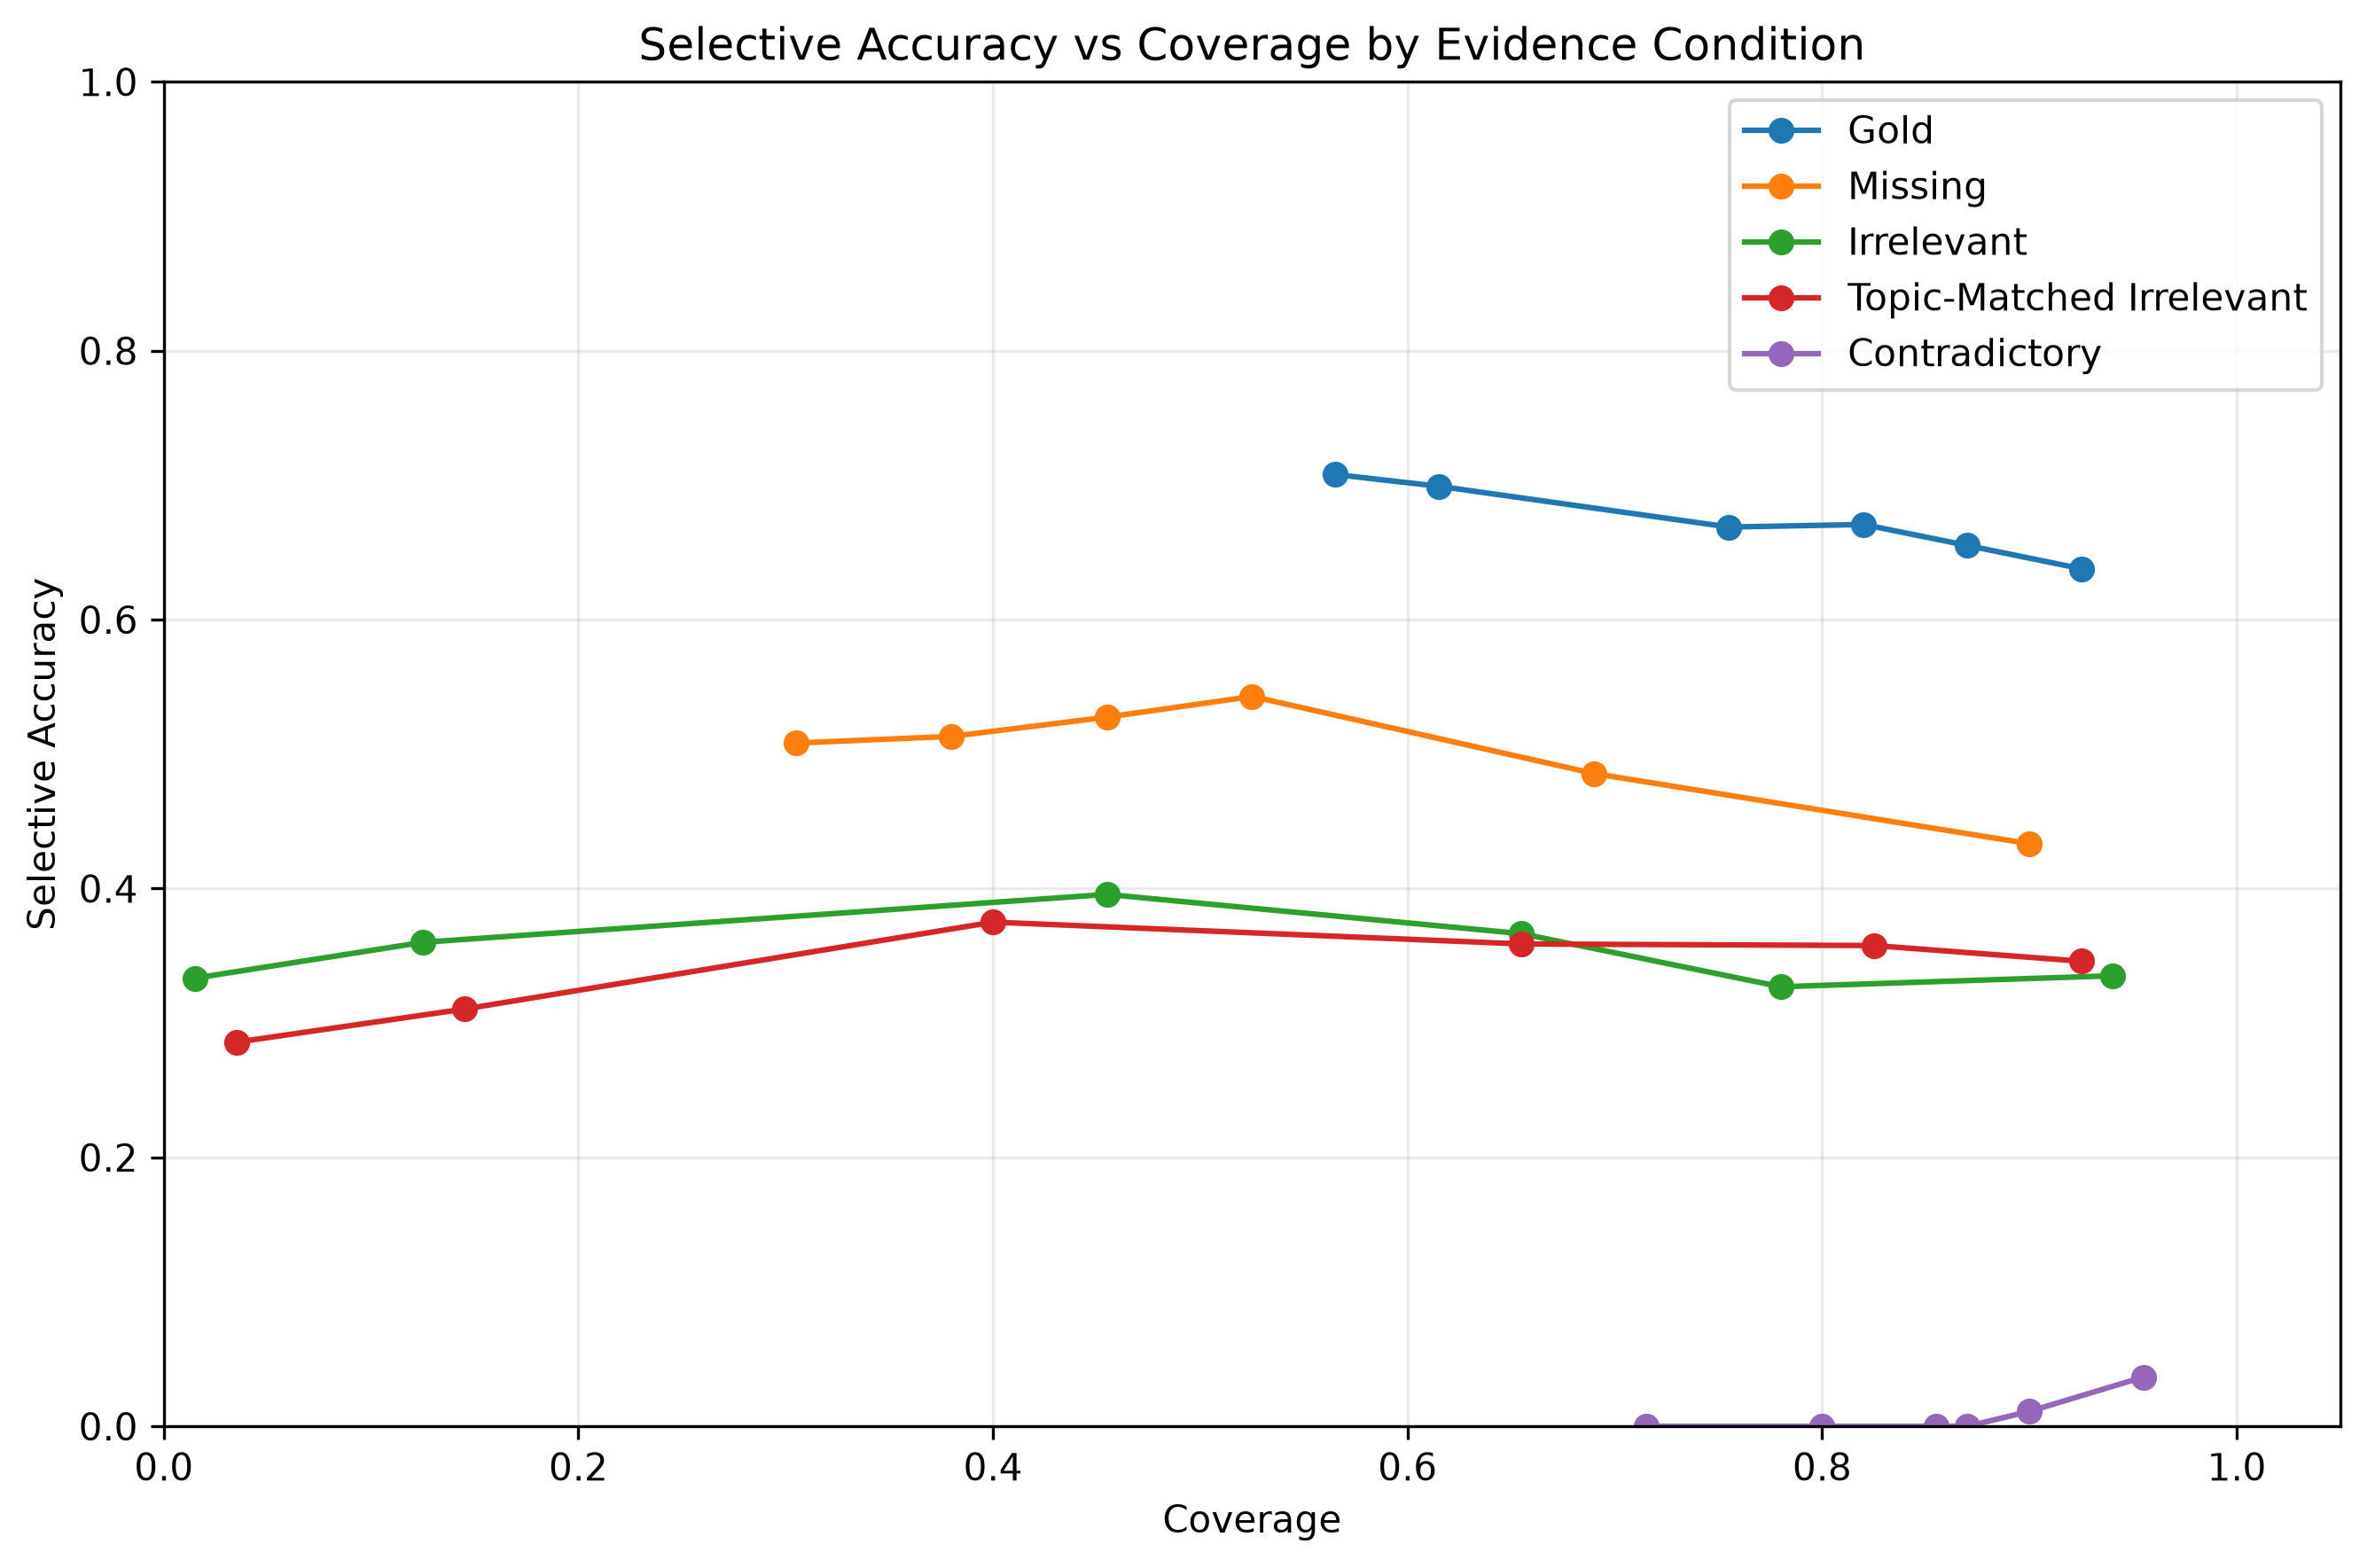
\includegraphics[width=\columnwidth]{../figures/qwen25_condition_abstention_curves.png}
\caption{Selective accuracy versus coverage by evidence condition.}
\label{fig:condition_abstention}
\end{figure}

This demonstrates that simple confidence-based abstention cannot reliably identify contradiction-induced failure.

Overall selective accuracy changed only modestly as coverage decreased. This is consistent with the observation that some of the most harmful predictions were also among the most confident.

\section{Discussion}

\subsection{Correct Evidence Improves Biomedical QA}

The results demonstrate that retrieval can provide substantial benefit when the evidence is appropriate.

Gold evidence increased accuracy from 45.0\% without context to 62.0\%. The answer-flip analysis also showed a net improvement of 34 questions under gold evidence.

This supports the central motivation of RAG: external evidence can improve language-model reasoning when the retrieved information is relevant and reliable \cite{lewis2020rag}.

However, the experiments also demonstrate that this benefit should not be interpreted as a general property of retrieval.

\subsection{Poor Evidence Can Be Worse Than No Evidence}

All degraded evidence conditions performed below the gold condition.

Missing evidence also performed below the no-context baseline. Irrelevant and topic-matched irrelevant evidence produced even larger reductions in accuracy.

This suggests that a language model may attempt to incorporate contextual information even when that information does not provide useful support for the answer.

The topic-matched irrelevant condition is particularly important because it represents a failure that may be difficult to detect using simple keyword or semantic similarity. Evidence may appear relevant to the same biomedical topic while still failing to support the actual question.

Therefore, retrieval relevance alone may not be sufficient. Evidence should also be assessed for answer-level usefulness.

\subsection{Contradiction Is the Most Severe Failure Mode}

Contradictory evidence produced the strongest degradation.

Accuracy fell to 6.5\%, representing a dramatic decline relative to both the gold and no-context conditions.

The answer-flip analysis showed 87 harmful flips and only 10 helpful flips, producing a net change of -77.

This indicates that the model often followed contradictory contextual evidence even when its no-context answer had previously been correct.

The contradictory condition was synthetically constructed and therefore represents an intentionally severe stress test. Nevertheless, it provides evidence that a language model can be highly sensitive to misleading retrieved context.

\subsection{High Confidence Does Not Guarantee Reliability}

The most important uncertainty finding was that contradictory evidence produced the highest mean confidence.

The model achieved mean confidence of approximately 0.909 under contradiction despite achieving only 6.5\% accuracy.

In comparison, gold evidence produced slightly lower confidence of approximately 0.872 despite much higher accuracy.

This reverses the relationship that would be desirable in a safety-oriented system.

Ideally,

\begin{equation}
\text{poor evidence}
\rightarrow
\text{greater uncertainty}
\rightarrow
\text{possible abstention}.
\end{equation}

Instead, the contradictory condition frequently produced

\begin{equation}
\text{poor evidence}
\rightarrow
\text{high confidence}
\rightarrow
\text{incorrect answer}.
\end{equation}

This creates a particularly challenging safety problem because the system may provide unreliable answers without displaying uncertainty.

\subsection{Confidence-Based Abstention Is Insufficient}

Selective classification is intended to improve reliability by rejecting low-confidence predictions \cite{geifman2017selective}.

The present results show that this strategy can be limited when errors are caused by misleading evidence.

At a confidence threshold of 0.90, contradictory predictions had 80.0\% coverage but 0\% selective accuracy.

Increasing the confidence threshold therefore failed to reject the most severe evidence-induced errors.

This indicates that biomedical RAG systems may require evidence-aware abstention rather than model-confidence-only abstention.

Potential signals could include retrieval score, question-evidence semantic consistency, contradiction detection, evidence-source agreement, evidence provenance, and cross-document verification.

\subsection{Biomedical Implications}

Biomedical RAG systems are attractive because retrieved scientific literature can provide current and verifiable information.

However, the present results demonstrate that retrieval can introduce a new failure pathway.

A system may retrieve a document that is semantically related but not actually supportive of the target question. It may also encounter conflicting findings or evidence that reflects a different population, intervention, outcome, or study design.

If the language model treats all supplied evidence as equally trustworthy, the final answer may become less reliable.

Biomedical RAG systems should therefore consider evidence quality as a separate component of system reliability.

This may require mechanisms that evaluate relevance, sufficiency, provenance, consistency, and contradiction before generation.

\subsection{Class Imbalance and Metric Interpretation}

The class distribution was imbalanced, with the \textit{maybe} category substantially less frequent than \textit{yes} and \textit{no}.

For this reason, accuracy alone does not fully describe model performance.

Balanced accuracy and macro-F1 provide additional information by reducing the dominance of majority classes.

The difference between standard accuracy and these class-balanced metrics suggests that performance was uneven across labels.

Future work could therefore investigate label-specific sensitivity to evidence perturbation, particularly for the less frequent \textit{maybe} category.

\subsection{Limitations}

This study has several limitations.

First, only one instruction-tuned language model was evaluated. Qwen2.5-1.5B-Instruct is relatively small compared with many current LLMs, and larger models may respond differently to evidence perturbations.

Second, the controlled experiment used 200 PubMedQA development questions. Although each question was evaluated under multiple evidence conditions, the number of unique biomedical questions remains limited.

Third, the contradictory evidence was synthetic. This provided a controlled stress test but does not capture the full complexity of genuine disagreement between biomedical studies.

Fourth, the confidence score was obtained by normalizing logits associated with the three allowed labels. These values represent relative model preference among \textit{yes}, \textit{no}, and \textit{maybe}; they are not fully calibrated probabilities over all possible language-model outputs.

Fifth, BM25 was the main retrieval baseline. Dense or hybrid retrieval systems may produce different retrieval-error profiles \cite{karpukhin2020dpr}.

Finally, the controlled evidence experiments were conducted on the development partition. A final held-out test evaluation would provide stronger evidence regarding generalization.

\subsection{Future Work}

Future work should evaluate multiple model families and model sizes.

The evidence-quality framework could also be extended to naturally conflicting biomedical literature, where disagreement may arise from differences in study design, patient population, sample size, intervention, or outcome definition.

Retrieval could be expanded beyond BM25 to include dense and hybrid retrieval.

Another important direction is explicit evidence-quality estimation. A separate model could assess whether evidence is relevant, sufficient, contradictory, or unsupported before passing it to the generator.

Multi-document consistency analysis may also improve reliability by comparing claims across several retrieved studies rather than relying on a single passage.

Biomedical RAG systems may ultimately require a combined decision rule based on both model uncertainty and evidence quality rather than confidence alone.

\section{Conclusion}

This study evaluated how controlled evidence quality affects biomedical retrieval-augmented question answering.

Gold evidence improved accuracy from 45.0\% without context to 62.0\%.

Missing, irrelevant, topic-matched irrelevant, and contradictory evidence reduced performance, demonstrating that retrieval does not inherently improve biomedical question answering.

The most severe failure occurred under contradictory evidence, where accuracy fell to 6.5\% while mean confidence increased to approximately 0.909.

Simple confidence-based abstention did not detect this failure. At a confidence threshold of 0.90, the model retained 80.0\% of contradictory predictions while achieving 0\% selective accuracy.

These results highlight the importance of evaluating retrieved evidence before treating a biomedical RAG answer as trustworthy. Reliable biomedical RAG systems should therefore combine strong retrieval with evidence-quality assessment, contradiction detection, provenance checking, and evidence-aware uncertainty mechanisms.

\bibliographystyle{IEEEtran}
\bibliography{references}

\end{document}